\chapter{Cài đặt \& Môi trường làm việc}

% Nếu bạn nghĩ tự động hóa là thứ gì đó phức tạp, đòi hỏi hàng giờ lập trình hay một bộ óc thiên tài, thì chương này sẽ khiến bạn phải nghĩ lại. Với n8n, bạn không cần phải là Tony Stark để xây dựng một Jarvis cá nhân – bạn chỉ cần một chút tò mò và vài phút rảnh rỗi.

Nếu bạn từng nghĩ rằng tự động hóa chỉ dành cho các lập trình viên kỳ cựu, những bộ óc thiên tài hay những người làm việc trong phòng lab của Tony Stark, thì chương này sẽ khiến bạn phải nhìn lại. Sự thật là: với n8n, bạn không cần đến một đội ngũ kỹ sư, không cần phải ngồi gõ hàng trăm dòng mã, và càng không cần phải “nạp não” với những khái niệm lập trình phức tạp. Bạn chỉ cần một chiếc máy tính, một chút tò mò, và một chút thời gian giữa giờ cà phê.

Hãy bắt đầu bằng việc cài đặt n8n. Tôi sẽ dẫn bạn qua hai con đường: dùng phiên bản đám mây để thử ngay lập tức, hoặc tự lưu trữ trên máy tính nếu bạn muốn kiểm soát hoàn toàn. Đừng lo, quá trình này đơn giản đến mức bạn sẽ hoàn thành trước khi tách trà của bạn nguội đi.


\section{Cài đặt trên Windows, macOS, Linux}

\section{Chạy trên Cloud}
Truy cập trang chủ của \href{n8n.io}{n8n.io}, làm theo các hướng dẫn để đăng ký tài khoản, không cần cấu hình server, trả phí định kỳ.

- Điền đầy đủ các thông tin cần thiết, email, username, password, account\_name - domain khi sử dụng N8N. 

$\Rightarrow$ Đăng ký xong có ngay 14 ngày sài free để mọi người trải nghiệm dịch vụ nha. Sau đó cứ theo mức phí ở phần pricing mà trừ tiền nha :))

\section{Cài bằng node trên AWS EC2}

Bạn biết gì không, mỗi tài khoản AWS mới tạo sẽ được miễn phí một số tài nguyên. Mỗi tháng bạn sẽ có 750h free dùng t2.small (1v CPU, 2GB Ram). Vì vậy việc dùng AWS EC2 cx là một lựa chọn khá hợp lý.

Trước tiên bạn hãy khởi tạo một con EC2 t2.micro với 8GB bộ nhớ (EBS được free 30GB/tháng). Sau đó connect tới server đó và chạy các lệnh sau

- Lệnh tải n8n

\begin{lstlisting}
sudo npm install n8n
\end{lstlisting}

- Lệnh tắt mã hóa cookie

\begin{lstlisting}[language=bash]
export N8N_SECURE_COOKIE=false
\end{lstlisting}

- n8n thường chạy trong Terminal, nhưng nếu bạn thoát Terminal hoặc khởi động lại máy tính, n8n sẽ ngừng hoạt động. Để giải quyết vấn đề này, chúng ta có thể sử dụng một ứng dụng có tên PM2 để chạy n8n như một dịch vụ kể cả có tắt terminal thì nó vẫn hoạt động. 

\begin{lstlisting}[language=bash]
sudo npm install -g pm2
\end{lstlisting}

- Lệnh chạy n8n:
\begin{lstlisting}[language=bash]
pm2 start n8n --name n8n
\end{lstlisting}

- Lệnh dừng n8n:
\begin{lstlisting}[language=bash]
pm2 stop n8n
\end{lstlisting}

Truy cập giao diện web thông qua trình duyệt (thường là http://localhost:5678 hoặc http://ip:5678).



\subsection{Cài bằng Docker}
Oke nếu pro ko có Cloud, không sao bạn hoàn toàn có thể cài trên máy tính cá nhân. Và tất nhiên để cho gọn thì chúng ta hãy nghĩ đến container

- Tạo file docker-compose.yml mẫu:
\begin{lstlisting}
services:
  n8n:
    image: n8nio/n8n
    restart: unless-stopped
    ports:
      - "5678:5678"
    environment:
      - N8N_BASIC_AUTH_ACTIVE=true
      - N8N_BASIC_AUTH_USER=admin
      - N8N_BASIC_AUTH_PASSWORD=pass
      - N8N_HOST=localhost
      - N8N_PORT=5678
      - N8N_PROTOCOL=http
      - N8N_SECURE_COOKIE=false
    volumes:
      - n8n_data:/home/node/.n8n

volumes:
  n8n_data:
\end{lstlisting}

- Khởi động docker: 

\begin{lstlisting}
    docker-compose up -d
\end{lstlisting}

Do là dùng VPS nên có thể dung NGROK để cấp domain cho ip hiện tại. Do ip thì khó auth với các dịch vụ khác như facebook, google hơi khó.

\section{Cách cứu vãn trong trường hợp quên password n8n}

Kiểu gì cũng có mấy ông bà nào đó lập cái tài khoản xong quên mất. Dùng cloud thì quên mật khẩu dễ dàng. Còn nếu bạn dùng self-host thì sao :))

$\rightarrow$ Dùng CLI 

\begin{enumerate}
    \item Đối với cài bằng node chỉ việc mở terminal lên và chạy lệnh

\begin{lstlisting}[language = Bash]
n8n user-management:reset
\end{lstlisting}

Sau đó khởi động lại n8n là được

    \item Đối với docker

\begin{itemize}
    \item[-] Xem ID của container chứa n8n
\begin{lstlisting}
docker ps
\end{lstlisting}

\begin{lstlisting}
huyvv@server:~$ docker ps
CONTAINER ID   IMAGE       COMMAND   CREATED      STATUS      PORTS               NAMES
f3b82a9435e5 n8nio/n8n "tini -- /docker-entrypoint.sh ..." 3 days ago Up 3 days 0.0.0.0:5678->5678/tcp, [::]:5678->5678/tcp n8n-1
\end{lstlisting}


$\rightarrow$ f3b82a9435e5 là ID của container chứa n8n

\item[-] Truy cập vào container đó
\begin{lstlisting}
docker exec -it f3b82a9435e5 /bin/sh
\end{lstlisting}

\item[-] Chạy lệnh reset tài khoản
\begin{lstlisting}
n8n user-management:reset
\end{lstlisting}
\end{itemize}
\item[-] Tắt và khởi động lại container
\begin{lstlisting}
docker compose down
docker compose up -d
\end{lstlisting}
\end{enumerate}






\newpage

\section{Tổng quan giao diện n8n}

Sau khi cài đặt thành công đây là giao diện ban đầu:

\begin{figure}[htbp]
    \centering
    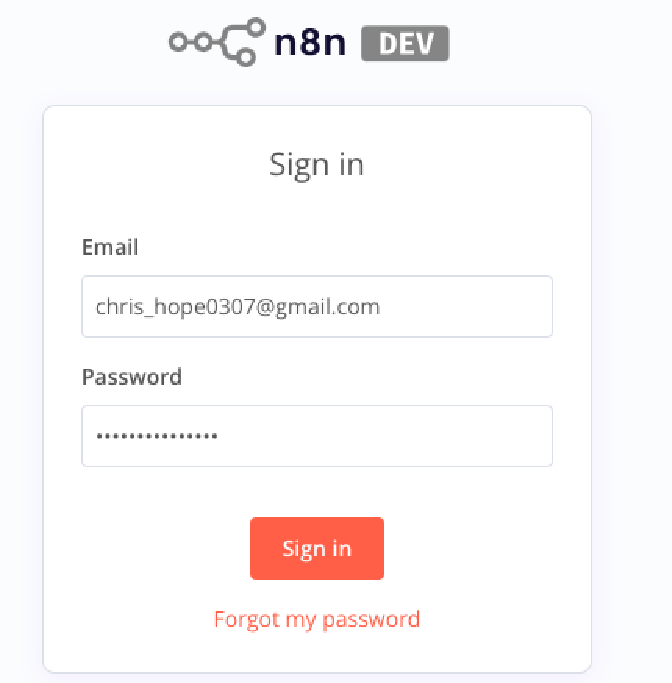
\includegraphics[width=0.8\linewidth]{Chap1-7/login.pdf}
    \caption{Giao diện đăng nhập}
\end{figure}

Editor UI trong n8n là một giao diện trực quan giúp bạn dễ dàng tạo quy trình tự động hóa bằng cách kết nối các node. Cách tiếp cận này lấy cảm hứng từ ngành công nghiệp phim ảnh và truyền hình, nơi mà nhiều công cụ sử dụng hệ thống node-based để xử lý dữ liệu một cách trực quan.

Nhìn lên trên bên trái, bạn sẽ thấy một biểu tượng >, nhấn vào đó để mở rộng menu chính của n8n.

Trước khi đi sâu vào từng tính năng, chúng ta sẽ làm quen với giao diện tổng thể để có thể dễ dàng điều hướng và thao tác. Khi đã thành thạo, bạn sẽ nhanh chóng xây dựng được những quy trình tự động hóa mạnh mẽ mà không cần viết code phức tạp.

Cùng xem menu này có những gì
\begin{itemize}
    \item New: Tạo một workflow mới.

    \item Open: Mở một workflow đã có sẵn.

    \item Save: Lưu thay đổi vào workflow hiện tại.

    \item Save As: Lưu workflow hiện tại với một tên mới.

    \item Rename: Đổi tên workflow.

    \item Delete: Xóa workflow hiện tại.

    \item Download: Tải xuống workflow dưới dạng file JSON.

    \item Import from URL: Nhập workflow từ một URL.

    \item Import from File: Nhập workflow từ một file JSON.

    \item Settings: Cấu hình cài đặt cho workflow hiện tại.
\end{itemize}

\textit{Lưu ý: Đừng quên \textbf{SAVE} lại workflow nếu không công sức brainstorm của pro sẽ bay màu đó :)).}

\textbf{Menu Credentials}

Menu này có hai tùy chọn:
\begin{itemize}
    \item New: Tạo một credential mới.

    \item Open: Mở một credential đã có sẵn.
\end{itemize}

n8n cho phép bạn kết nối với nhiều ứng dụng, dịch vụ và API khác nhau. Nhiều ứng dụng yêu cầu credentials để xác thực quyền truy cập. n8n hỗ trợ mã hóa và lưu trữ các credentials này trong cơ sở dữ liệu, giúp bạn có thể sử dụng lại dễ dàng khi tạo workflows mới.

\textbf{Tab Executions}

Tab này mở một cửa sổ (modal) hiển thị danh sách các lần thực thi của workflows. Bạn cũng có thể lọc executions theo tên và trạng thái.
\section{Nguyên tắc làm việc với n8n}

\begin{itemize}
    \item Hiểu rõ luồng làm việc: Dữ liệu đi từ đâu đến đâu, nó sẽ làm gì trong cái workflow đấy cũng như logic của nó. Workflow phải tối ưu ngắn hiệu quả. Đảm bảo tính nhất quản của dữ liệu trong suốt quy trình. Tránh các bước trung gian không cần thiết để giảm thiểu độ trễ và tài nguyên hệ thống. 
    \item Sử dụng trigger đúng cách: đặt lịch để workflow chạy, nhận dữ liệu trả về từ API, trigger từ các ứng dụng bên ngoài 
    \item Tận dụng các node trước để tối ưu workflow
    \item Kết hợp các nguồn API, webhook bên ngoài để mở rộng workflow 
    \item Quản lý lỗi hiệu quả. Báo lỗi khi workflow xảy ra sự cố. Triển khai node Error Trigger để phát hiện và xử lý các lỗi runtime
\end{itemize}

\newpage
\section{Tối ưu workflow}
\begin{figure}[htbp]
    \centering
    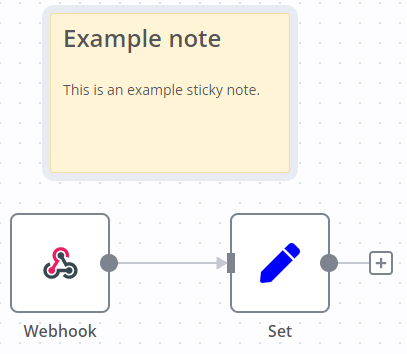
\includegraphics[width=0.8\linewidth]{Chap1-7/sticky-note.png}
    \caption{Sticky note}
\end{figure}

Để tránh trường hợp mà tạo xong workflow méo hiểu mình vừa kéo thả cái gì thì mình nghĩ mọi người nên chú ý các điều sau:
\begin{itemize}
    \item Thiết kế workflow càng dễ càng tốt
    \item Thêm note giải thích chi tiết (Shift + S)
    \item Làm đến đâu giải thích đến đấy
\end{itemize}


\section{Cách import, export worflow}
Tính năng này sinh ra nhằm mục tải worflow của bạn dưới dạng json và backup nó vào trong máy tính local hoặc push lên github để lưu trữ. Sau nay khi cần restore lại thì bạn chỉ cần upload lại 

\begin{itemize}
    \item Nhấn vào nút ba chấm trên cùng góc trái sau đó chọn "\textbf{Download}"
    \item Tương tự chọn "\textbf{Import from file or url} để import lại workflow đã lưu 
\end{itemize}